\subsection{Analysis Based on Method Strategy}
To further investigate the impact of translation granularity on the performance of large language models, we introduced a translation strategy based on individual methods and conducted a comprehensive data analysis of its results. This strategy involves extracting each Java method independently and instructing the model to translate it into the corresponding C++ method. This chapter will detail the overall performance under this strategy, compare the performance of different models, and conduct a horizontal comparison with the previously discussed class-based translation strategy to reveal how different strategies affect model translation behavior and hallucination patterns.

\subsection{Overall Performance}
\subsubsection{Overall Correctness Rate/Error Rate}
When translating the dataset using the method strategy, a total of 2121 methods were processed. Among them, 1521 methods were translated correctly, while 600 contained errors, resulting in an overall correctness rate of 71.71\% and an error rate of 28.29\%.

\begin{table}[H]
  \centering
  \label{tab:translation-stats}
  \begin{tabular}{lrr}
    \hline
    Metric                         & Quantity & Proportion (\%) \\
    \hline
    Correctly Translated Methods   & 1521     & 71.71           \\
    Incorrectly Translated Methods & 600     & 28.29           \\
    \hline
  \end{tabular}
\end{table}

The overall correctness rate of the method strategy (71.71\%) is significantly higher than that of the class strategy (60.73\%), an absolute improvement of about 11 percentage points. This result indicates that breaking down the translation task into smaller, more focused units (individual methods) can effectively increase the probability of LLMs generating correct code. When the model only needs to focus on the internal logic of a single method, the complexity is significantly reduced, thereby lowering the likelihood of errors. This demonstrates that refining the translation granularity is an effective way to enhance LLM performance in code migration tasks.

\subsubsection{Performance w.r.t LLMs.}
Under the method translation strategy, we also compared the performance of the GPT and DeepSeek models:

\begin{itemize}[leftmargin=1.5em]
    \item \textbf{GPT: }GPT processed a total of 1089 methods, with 782 correct and 307 incorrect, for a correctness rate of 71.81\%.
    \item \textbf{DeepSeek: }DeepSeek processed a total of 1032 methods, with 739 correct and 293 incorrect, for a correctness rate of 71.61\%.
\end{itemize}
\begin{figure}[H]
  \centering
  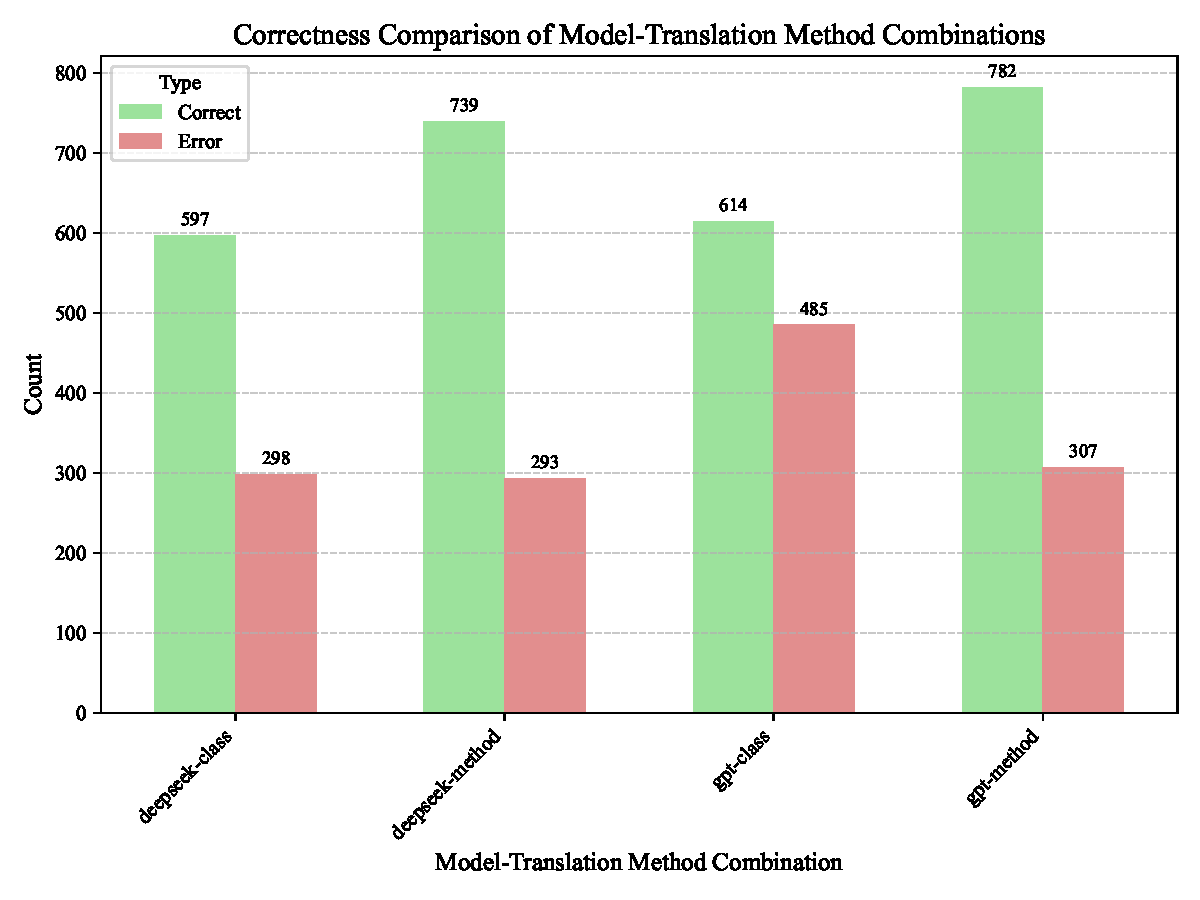
\includegraphics[width=0.5\textwidth]{pdf/Model_Translation_Method_Correctness_Comparison_Bar_Chart.pdf}
\end{figure}

This result presents a stark contrast to the model performance under the class strategy. In the class strategy, DeepSeek's correctness rate (66.70\%) was significantly superior to GPT's (55.87\%). However, under the method strategy, the two models' correctness rates are surprisingly close, with almost no significant difference; GPT's performance is even slightly better.

This reversal of trends indicates that translation granularity is a key variable affecting the relative performance of the models. DeepSeek shows an advantage when handling more complex, context-rich class-level translation tasks, which may be due to its stronger ability to understand the overall code structure. However, when the task is simplified to a method-level translation with limited contextual information, GPT demonstrates equivalent or even slightly stronger competitiveness. This suggests that GPT is highly efficient at handling local, independent logic fragments, while DeepSeek's advantages are not fully realized when information is constrained.

\subsubsection{Performance w.r.t Projects.}
Under the method strategy, we also analyzed the translation performance across the five projects to assess how the change in translation granularity affects different types of projects.

\begin{table}[H]
  \centering
  \begin{tabular}{lccccc}
    \hline
    Project Name & File Count & Correct Methods & Erroneous Methods & Correctness Rate &  Dominant Error Types (Count) \\
    \hline
    Cookie & 9 & 137 & 53 & 72.1\% & Improper memory management(18), Method partially unimplemented (partially missing)(14) \\
    EnableJUnit4MigrationSupport & 32 & 333 & 254 & 56.7\% & Method not implemented (entirely missing)(155), Referencing non-existent classes(84) \\
    HoverMenuService & 9 & 195 & 25 & 88.6\% & Referencing non-existent methods or member variables(14) \\
    IntMath & 7 & 135 & 64 & 67.8\% & Method not implemented (entirely missing)(40) \\
    NoopIndexDAO & 21 & 724 & 205 & 77.9\% & Method not implemented (entirely missing)(187) \\
    \hline
  \end{tabular}
\end{table}

The correctness rate for all projects improved under the method strategy. The most significant improvements were seen in HoverMenuService (jumping from 53.7\% to 88.6\%) and IntMath (from 47.8\% to 67.8\%). This strongly proves that decomposing the task into smaller units (methods) effectively reduces translation complexity, with more pronounced effects on projects that performed poorly under the class strategy.
The change in translation granularity also led to a shift in error patterns. For instance, the primary error in the HoverMenuService project shifted from "Method not implemented (entirely missing)" under the class strategy to "Referencing non-existent methods or member variables" under the method strategy. This highlights a critical issue: when the context is limited to a single method, the model is less likely to omit the implementation, but its lack of awareness of the entire class makes it more prone to hallucinate when handling inter-method call relationships.
Despite the improved correctness rate, the EnableJUnit4MigrationSupport project (56.7\%) still performs the worst. Its errors remain concentrated in "Method not implemented (entirely missing)" and "Referencing non-existent classes," indicating that even when the task is decomposed, LLMs still face significant challenges in inferring missing context and dependencies for inherently complex projects.
The correctness rate of the Cookie project decreased under the method strategy, which contradicts the general trend of improvement in other projects. Its primary error is "Improper memory management," which may suggest that the project contains many low-level operations requiring careful memory handling. Under the class strategy, the full context helps the model understand these operations, whereas, under the method strategy, the lack of information leads to more of these subtle logical errors.
In conclusion, the method strategy generally improves the translation correctness rate across projects by reducing task complexity. However, this strategy also amplifies the model's hallucination problem when dealing with local dependencies and may negatively affect specific code (such as memory management) that relies on a complete context.

\subsubsection{Error Type Distribution}
Among the 600 errors produced by the method strategy, "Method not implemented (entirely missing)" remains the most numerous error type, with 390 instances, accounting for 65\% of all errors. This is followed by "Referencing non-existent classes," with 92 instances, making up 15.33\%. Other error types such as "Method partially unimplemented (partially missing)" (28 instances) and "Referencing non-existent methods or member variables" (27 instances) also account for a certain proportion, but their numbers are small compared to the first two categories.
\begin{figure}[H]
  \centering
  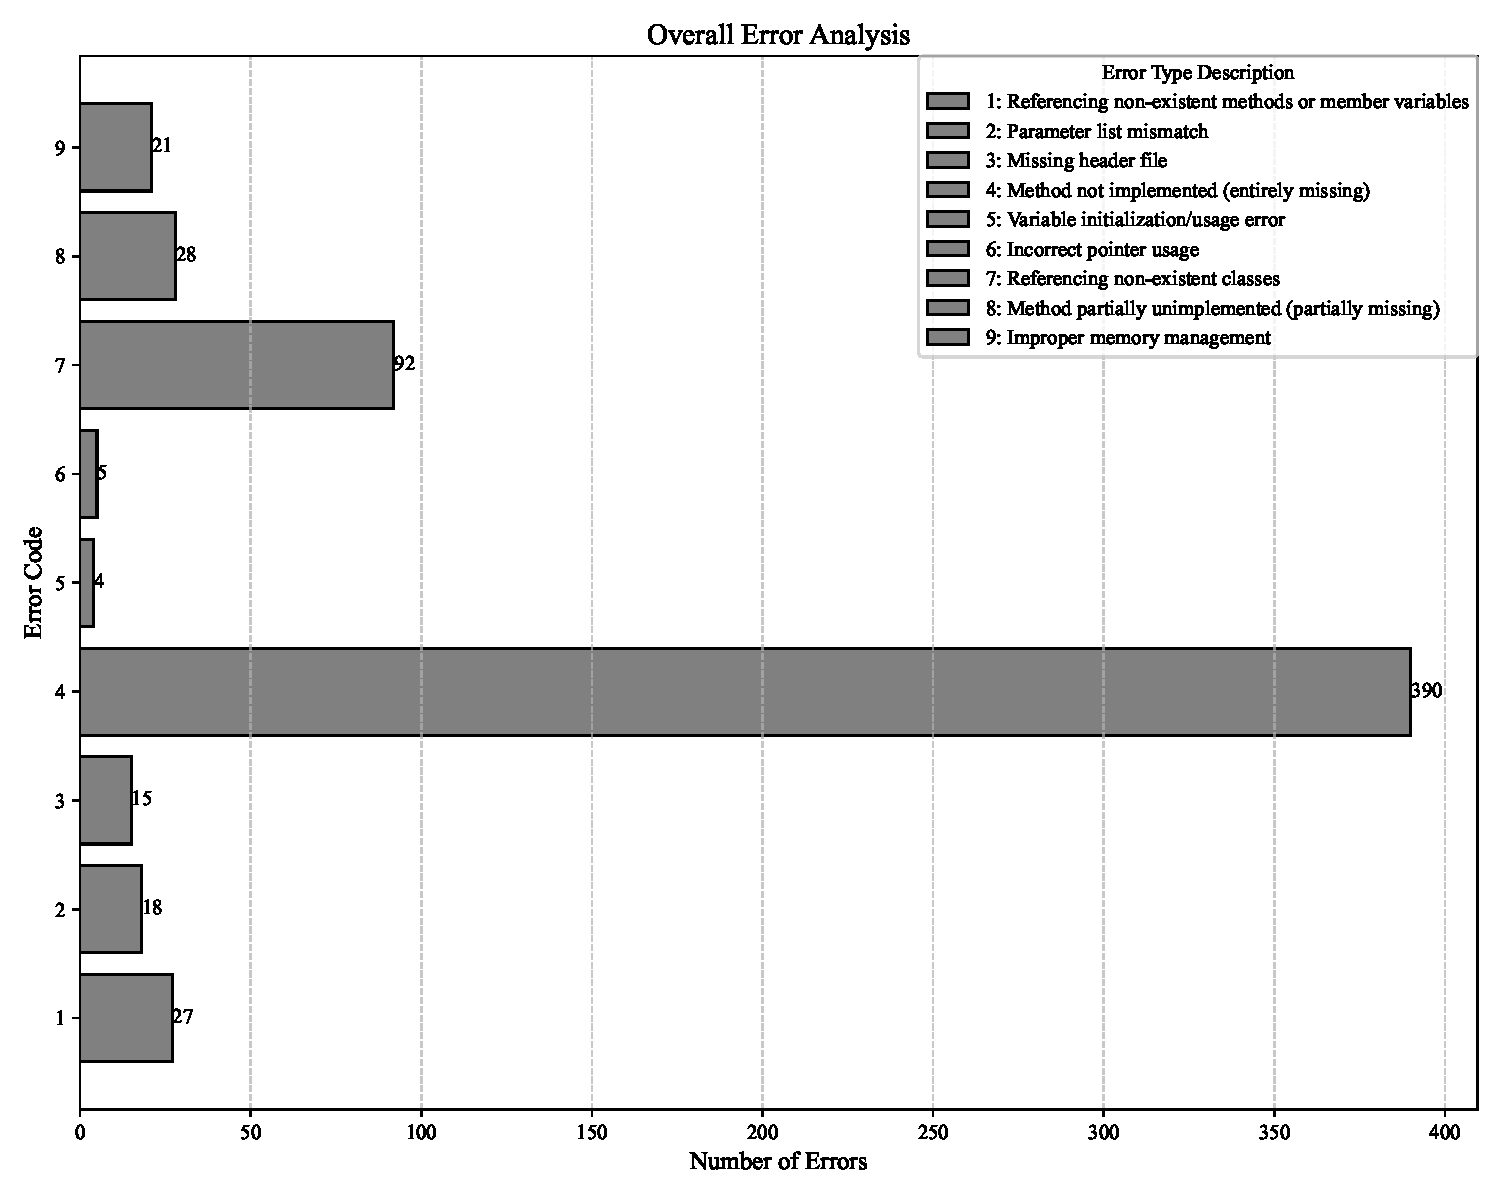
\includegraphics[width=0.5\textwidth]{pdf/Overall Error Analysis1.pdf}
\end{figure}

Similar to the error distribution of the class strategy, "Method not implemented (entirely missing)" is also the primary form of hallucination in the method strategy. However, it is worth noting that the proportion of this error in the method strategy (65\%) is much higher than its proportion in the class strategy (approximately 51.53\%). This reveals a key phenomenon: when contextual information is limited to a single method, if the model cannot resolve the method's external dependencies (such as other classes, global variables, etc.), it is more inclined to abandon code generation altogether rather than attempting a potentially incorrect implementation. This "safe" failure strategy, while leading to a large number of missing methods, may also be one of the reasons for its higher overall correctness rate, as it avoids generating more functionally incorrect code containing other types of errors.

Furthermore, the relatively high proportion of "Referencing non-existent classes" errors (15.33\%) highlights the significant challenges models face in inferring and reconstructing external dependencies when a complete class definition context is lacking.

\subsubsection{Error Type Distribution by Model}
Although the two models have similar overall correctness rates under the method strategy, their error patterns reveal distinct weaknesses.

\begin{itemize}[leftmargin=1.5em]
    \item \textbf{GPT Error Distribution: }Among its 307 errors, "Method not implemented (entirely missing)" is absolutely dominant, with 239 instances, accounting for 77.85\% of its own errors. In contrast, other error types such as "Referencing non-existent classes" (19 instances) and "Referencing non-existent methods or member variables" (15 instances) are very few. This indicates that GPT's main failure mode in the method strategy is to give up on generation when faced with uncertainty.
    \item \textbf{DeepSeek Error Distribution: }Among its 293 errors, "Method not implemented (entirely missing)" is still the primary error, but its number (151 instances) is much lower than GPT's, accounting for 51.54\% of its own errors. However, DeepSeek shows a clear tendency for the "Referencing non-existent classes" error, with 73 instances, accounting for 24.91\% of its own errors, far higher than GPT's for the same error type.
\end{itemize}
\begin{figure}[H]
  \centering
  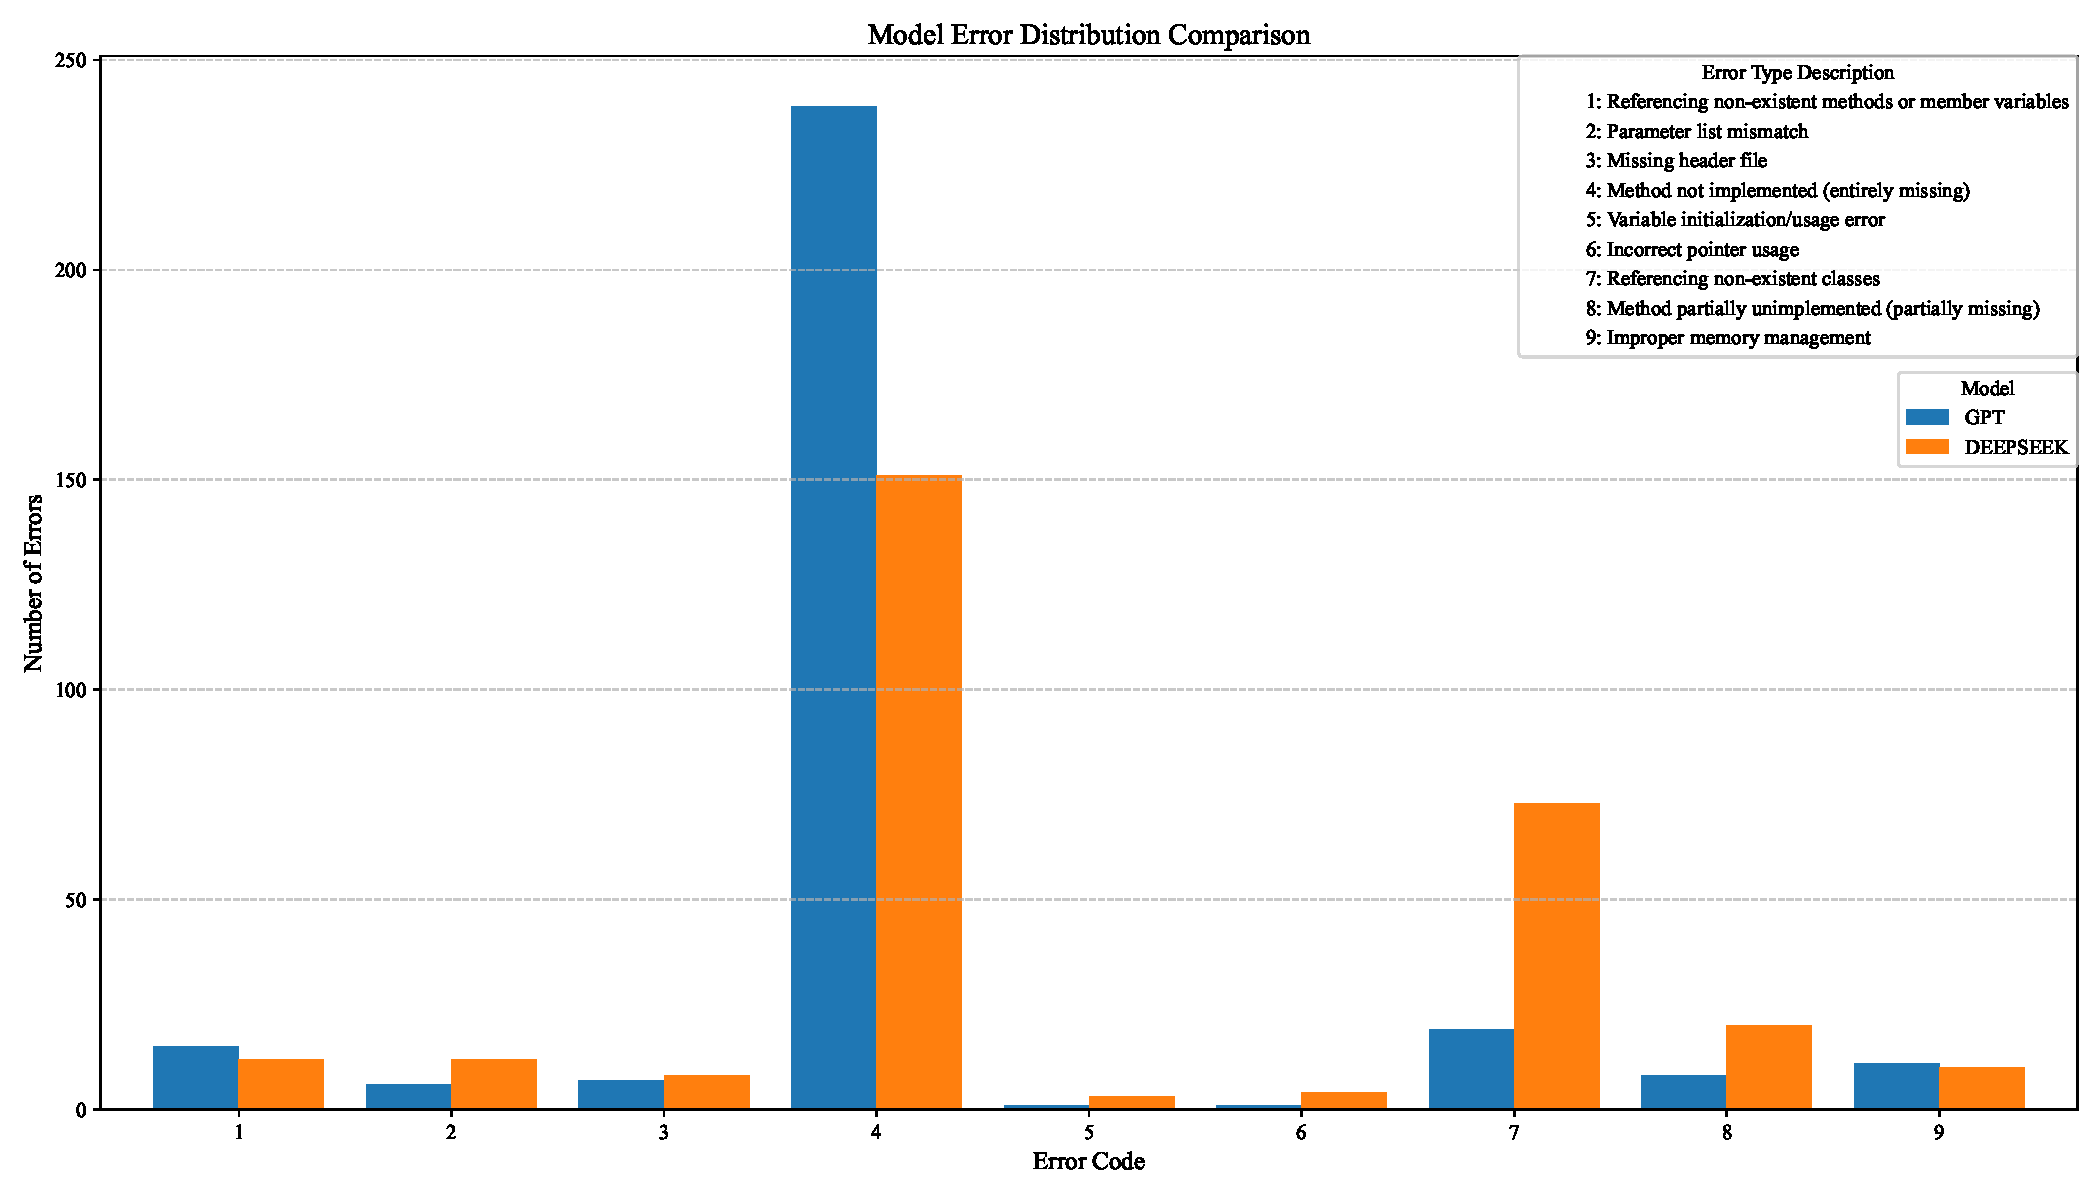
\includegraphics[width=0.5\textwidth]{pdf/Model Error Distribution Comparison1.pdf}
\end{figure}

This differentiated error pattern is highly instructive. In the method strategy, GPT's approach seems to be "better to have nothing than something bad"; when external dependencies are unclear, it is highly likely to choose not to generate any code. In contrast, DeepSeek is more "adventurous." It will more actively attempt to generate code, but due to the lack of sufficient context, it frequently produces hallucinations when inferring external class dependencies, i.e., "inventing" non-existent classes.

Looking back at the class strategy, both models had relatively few errors of "Referencing non-existent classes" (41 for GPT, 20 for DeepSeek) because the complete class definition provided more context. However, under the method strategy, this problem is drastically amplified for DeepSeek, indicating that when processing code snippets with incomplete contextual information, its issue with external dependency hallucinations is more severe than GPT's.

\subsection{Data Analysis Summary}
Through the data analysis of the method translation strategy and its comparison with the class strategy, we can draw the following conclusions:

\begin{itemize}[leftmargin=1.5em]
    \item \textbf{Translation Granularity Affects Overall Correctness Rate: }Refining the translation task from the class level to the method level can increase the LLM's translation correctness rate from about 61\% to about 72\%. This proves that optimizing LLM performance by decomposing task complexity is an effective strategy.
    \item \textbf{"Method not implemented" is the Core Hallucination Pattern: }Regardless of the granularity, "Method not implemented (entirely missing)" is the most dominant error type. In the method strategy, which has less contextual information, the models reinforce this "safe failure" strategy, leading to a further increase in the relative proportion of this error. This suggests that enhancing the models' ability to infer and complete code with incomplete information is a key direction for future research.
    \item \textbf{Relative Model Advantages and Weaknesses Vary with the Task: }DeepSeek performs better on complex, high-context class-level translations, while GPT can keep pace or even slightly surpass it on simple, low-context method-level translations. This shows that there is no universally superior model; the choice of model should depend on the specific task scenario and requirements. In low-context scenarios, GPT's main problem is a lack of implementation completeness (tending not to generate), while DeepSeek's main problem is dependency hallucination (tending to generate incorrect dependencies). This finding provides an important basis for the targeted use and improvement of different models. For example, when using DeepSeek for method-level translation, it is necessary to be particularly vigilant and design verification mechanisms to check whether its generated code references non-existent external dependencies.
\end{itemize}
